\documentclass[]{book}
\usepackage[english]{babel}
\usepackage{graphicx}
\begin{document}


\chapter{ICTP electronics}

\noindent Como se expuso anteriormente, los sistemas de detección de partículas cuentan con secciones encargadas de generar señales eléctricas que contienen la información física de interés del evento detectado. Dependiendo de la naturaleza del detector y de los objetivos del experimento, distintos elementos electrónicos pueden ser implementados a continuación. Sin embargo, el objetivo de estas etapas converge a preservar y transportar la mencionada información optimizando la relación señal/ruido. \\

\noindent Próxima al detector, se encuentra la etapa denominada front-end, que típicamente comprende electrónica analógica para la amplificación de la señal, shaping y discriminación, así como digitalización y transporte por cables. A continuación pueden encontrarse sistemas de más alto nivel como procesadores digitales y de adquisición de datos, que permiten transformar las señales y extraer la información necesaria para su posterior estudio. En la figura \ref{fig:generic_frontend} se observa un esquema genérico de la electrónica de front-end de un detector [Kolanoski].

\begin{figure}[h]
    \centering
    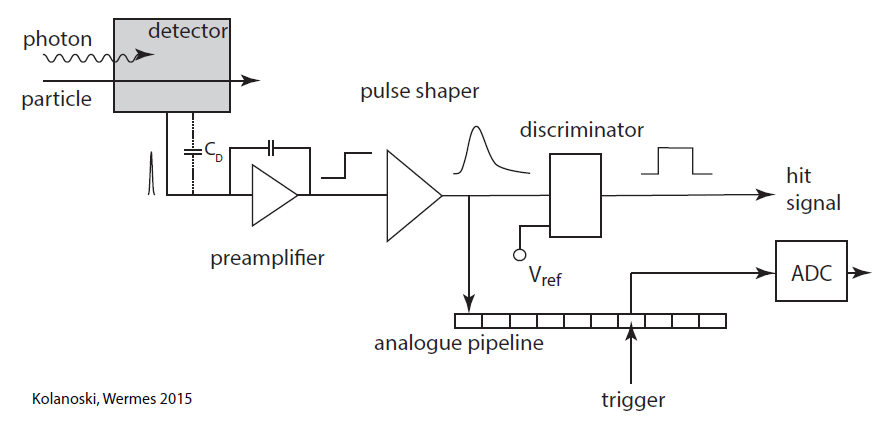
\includegraphics[width=0.7\textwidth]{typical_readout_electronics.PNG}
    \caption{Un esquema de electrónica de front-end típico, utilizado a menudo para la lectura de un
    detector, que incluye amplificación, conformación de impulsos, discriminación
    (aquí analógica) y digitalización (representada aquí por un ADC).}
    \label{fig:generic_frontend}

\end{figure}
    
\noindent Tal es el caso de los detectores GEM. Tras los fenómenos físicos consecuentes a la detección de una partícula, que se describen en el capítulo de física del detector, los electrones multiplicados son recogidos en un conjunto de electrodos, resultando una señal de corriente eléctrica que puede ser medida y analizada.\\

\noindent No obstante, las corrientes típicas medidas en la salida del detector pueden ser muy pequeñas, del orden de nanoamperios, lo que obstaculiza el uso de electrónica convencional para el procesamiento de la señal. Por lo tanto, es necesario implementar etapas de preamplificación y amplificación, hasta lograr señales con características adecuadas para su digitalización y el subsecuente procesamiento. A continuación, tanto los elementos de la etapa de front-end, como los de procesamiento digital utilizados en el presente trabajo serán explicados con detalle.

\subsection*{Front-end electronics}

\noindent Según la configuración de los electrodos de recolección de carga del detector, es posible sensar eventos en varios canales de lectura paralelamente, logrando una importante resolución espacial. Sin embargo, en este trabajo se desarrolla un sistema monocanal para la adquisición de datos de un detector GEM como versión mínima funcional. Los electrodos de salida del detector están conectados en paralelo y conducidos a una única conexión con un cable tipo X. Posteriormente, se conecta una resistencia en serie para permitir la medición de la caída de voltaje en sus terminales, lo que convierte la señal de corriente original del detector en una señal de voltaje que puede ser acondicionada.\\

%inlcuir fotografía de los terminales soldados y la resistencia en serie con el conector del cable

\noindent De acuerdo a [1], La función principal del preamplificador es captar la señal del detector sin deteriorar notablemente la relación señal/ruido inherente. Por ello, el preamplificador se ubica generalmente lo más cerca posible del detector para reducir la carga capacitiva sobre este, y los circuitos de entrada del preamplificador están diseñados para ajustarse a las características del detector. En particular, el sistema de preamplificación utilizado en este trabajo es el Ortec 142B, un dispositivo charge-sensitive diseñado para capacitancias de entrada de entre 100 y 400 pF. %inlcuir fotografía del preamp\\
%qué tantas especificaciones técnicas del preamp debería incluir aquí?

La señal de salida del preamplificador está caracterizada por... y teniendo en cuenta que el ADC tiene un rango de trabajo de ..., es necesario agregar una etapa de amplificación para imprimir en la señal una ganancia de x.\\

\noindent Como explica [2], la amplificación por etapas de una señal ofrece numerosas ventajas significativas. Principalmente, permite reducir el ruido generado en cada etapa individual, resultando en una señal final más limpia y menos propensa a la distorsión. Este método también mejora la estabilidad del sistema al distribuir la amplificación, evitando la saturación que podría ocurrir con una amplificación intensa en una sola etapa. Además, facilita el control preciso de la ganancia y la adaptación de impedancias entre diferentes componentes, lo cual mejora la eficiencia y la transferencia de la señal. La amplificación gradual es particularmente útil para manejar señales débiles, amplificándolas sin riesgo de distorsión. Asimismo, distribuye la carga térmica generada, disminuyendo el riesgo de sobrecalentamiento de los componentes. \\

%aquí seria necesario poner datos experimentales de la caracterización del detector, mostrando el factor de ganacia etc
%debería poner el desarrollo matemático de un charge-sensitive preamp? (lo tengo referenciado)

\noindent De esta manera, dando continuidad al recorrido de la señal después del preamplificador, se implementa un amplificador [referencia del amp NIM], hacer una caracterización similar a la del preamp y preguntar si sacar curvas experimentales y qué tantos datos técnicos del fabricante.\\

\noindent Teniendo en cuenta que el rango de operación del ADC es de [] mv (citar la datasheet del ADC), ya se cuenta con una señal que puede ser digitalizada.\\

\noindent Como explica [1], La digitalización de las señales provenientes de un detector es crucial debido a la precisión y flexibilidad que ofrece frente a los métodos analógicos tradicionales. Con el avance de los convertidores analógico-digitales (ADC) de alta velocidad y buena resolución desde los años 90, la posibilidad de procesar digitalmente los pulsos de los detectores se ha consolidado. Las ventajas de este enfoque incluyen una flexibilidad ilimitada en la elección de parámetros de conformación, mayor estabilidad al eliminar el riesgo de derivas debido a cambios de temperatura o voltaje, y la capacidad de realizar análisis más detallados con múltiples salidas de un mismo detector. Además, la manipulación digital no introduce ruido adicional y permite la implementación precisa de formas de pulso que serían difíciles o imposibles de lograr en circuitos analógicos. Sin embargo, una desventaja potencial es la limitación en la precisión del tiempo de detección, ya que los sistemas digitales están restringidos a la frecuencia de muestreo más cercana, lo que puede ser menos exacto que los métodos analógicos simples en aplicaciones que requieren una temporización muy rápida.\\

\noindent La función principal de un ADC (convertidor analógico-digital) es generar un código digital o número en su salida, que sea proporcional a la tensión analógica suministrada a su entrada. En un ADC genérico, las conversiones se realizan de forma continua a una frecuencia de reloj fija. Por ejemplo, un reloj de 500 MHz producirá 500 millones de muestras por segundo (MSPS), lo que equivale a una muestra cada 2 nanosegundos. En un ADC ideal, cada conversión de voltaje de entrada a código de salida es independiente, perfectamente lineal y ocurre instantáneamente. Sin embargo, las imperfecciones en los ADCs reales limitan tanto la frecuencia máxima de muestreo como la linealidad y la precisión de la conversión.




\subsection*{Sistema de adquisición y procesamiento}

\noindent 

\subsection*{References}
\begin{enumerate}
    \item Knoll, G F. (2000) Radiation Detection and Measurement, 3rd edition, John Wiley, New
    York.
    \item "Digital Signal Processing: Principles, Algorithms, and Applications" de John G. Proakis y Dimitris K. Manolakis.
\end{enumerate}

\end{document}